\documentclass[12pt]{article}					% Začátek dokumentu
\usepackage{../../MFFStyle}							% Import stylu

\begin{document}
\begin{priklad}[4.1]
	Zkonstruujte rozšířenou formu hry Kámen-nůžky-papír z Tabulky 1 a určete její sekvenční formu a lineární program k nalezení Nashových ekvilibrií této hry.

	\begin{center}
		\begin{tabular}{c|c|c|c}
			      & Kámen      & Nůžky      & Papír      \\ \hline
			Kámen & $( 0,  0)$ & $( 1, -1)$ & $(-1,  1)$ \\
			Nůžky & $(-1,  1)$ & $( 0,  0)$ & $( 1, -1)$ \\
			Papír & $( 1, -1)$ & $(-1,  1)$ & $( 0,  0)$
		\end{tabular}

		Tabulka 1: Hra Kámen-nůžky-papír v normálním tvaru
	\end{center}

	\begin{reseni}[Rozšířená forma]
		Díváme se na hru, jako by nejdříve volil jeden (BÚNO první) hráč a pak druhý (v rozšířené formě stejně má hráč informaci jen o tom, co dělal on).
		\vspace{-1.5em}
		
		\begin{center}
			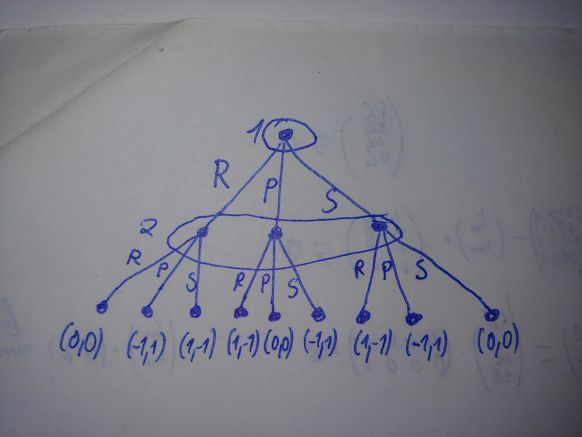
\includegraphics[width=0.35\textwidth]{ATH_DU4.jpg}
		\end{center}
		
		\vspace{-2.5em}
	\end{reseni}

	\begin{reseni}[Sekvenční forma]
		Sekvenční forma je čtveřice hráči-sekvence–užitek-omezení. Hráči jsou jasní, máme dva (BÚNO 1 a 2). Posloupnosti získáme přímočaře, množiny posloupností obou hráčů musí obsahovat prázdnou množinu a „poté co hráči zatím nic nezahráli“ (prázdná množina) si mohou vybrat buď kámen $(K)$, nůžky ($N$) nebo papír ($P$). Potom už hra skončila, takže žádný další člen do posloupnosti. Tedy $S_1 = S_2 = \{\O, K, N, P\}$.

		Užitkovou funkci udáme jako matice $A$ a $B$ mající v řádcích sekvence prvního hráče a ve sloupcích sekvence druhého. Řídíme se přesně listy v rozšířené formě (žádné listy $= 0$ nechávám prázdné, listy $(0, 0)$ značím $0$):
		$$ A = \bordermatrix{ & \O & K & N & P \cr \O &  &  &  & \cr K &  & 0 & 1 & -1 \cr N &  & -1 & 0 & 1 \cr P &  & 1 & -1 & 0 } \qquad
		  B = \bordermatrix{ & \O & K & N & P \cr \O &  &  &  & \cr K &  & 0 & -1 & 1 \cr N &  & 1 & 0 & -1 \cr P &  & -1 & 1 & 0 }. $$

		  Poslední člen čtveřice jsou podmínky na plán realizace. Víme $x(\O) = y(\O) = 1$. To pak rozdělujeme mezi možné tři stavy, takže
		  $$ y(K) + y(N) + y(P) = y(\O) = x(\O) = x(K) + x(N) + x(P). \qquad x ≥ 0 \land y ≥ 0. $$
	\end{reseni}

	\begin{reseni}[Lineární program]
		Podmínky přepíšeme do maticového tvaru:
		$$ E·¦x := \begin{pmatrix} 1 & 0 & 0 & 0 \\ -1 & 1 & 1 & 1 \end{pmatrix}·¦x = \begin{pmatrix} 1 & 0 \end{pmatrix} =: ¦e, \qquad ¦x ≥ ¦0. $$
		Stejně tak $F$ a ¦f, tedy $E = F$ a $¦e = ¦f$ a $¦y ≥ ¦0$. Nyní už máme vše, co je potřeba k lineárnímu programu uvedenému ve skriptech:
		$$ \max_{¦v, ¦x} ¦f·¦v, \text{ za podmínek } E¦x = ¦e \land F^T¦v - A^T¦x ≤ ¦0 \land ¦x ≥ ¦0. $$
		(První a třetí podmínku máme z postupu výše, $¦f·¦v$ nám říká, že bereme užitek v kořeni a druhá podmínka vlastně říká to, jak se šíří užitek z listů, kde ho známe, směrem ke kořeni.)
	\end{reseni}
\end{priklad}

\begin{priklad}[4.2]
	Předpokládejme, že v aukci prodáváme $k$ identických položek celkem $n > k$ kupujícím. Předpokládejme, že každý kupující může získat nanejvýš jednu položku. Jak vypadá příslušná varianta Vickreyovy aukce? Dokažte, že je DSIC.

	\begin{reseni}
		Zřejmě chceme prodat $k$ nejvyšším nabídkám, protože chceme aby Vickreyova aukce byla awesome (tj. podle bodu dva musíme maximalizovat sociální zisk). Inspirujeme se u $k = 1$, kde prodáváme nejvyšší nabídce za druhou nejvyšší nabídku. Budeme tedy prodávat za $k+1$-ní nejvyšší nabídku (za jednu z vyšších cen by se mohlo vyplatit vsázet méně než na kolik si to cením) $k$ nejvyšším nabídkám.

		Zřejmě užitek každého, kdo vsadí svoji hodnotu, je nezáporný, jelikož $k+1$-ní nabídka je nejvýše taková, jako $k$ nejvyšších. Takže druhý bod definice DSIC je splněna.

		Teď už zbývá, že vsadit svoji hodnotu je dominantní strategie. To znamená, že v žádném případě není lepší jiná strategie. Jiné strategie jsou dvě: vsadit méně a vsadit více. Pokud vsadím méně, tak svůj užitek nezvýším, neboť buď jsem už se svou hodnotou předmět nezískal, takže ho s menší nabídkou nezískám také (tj. z 0 na nulu), nebo jsem ho získal, ale za na mé nabídce nezávislou cenu, takže ho leda můžu nezískat (tj. z nezáporného na nulu).

		Pokud nabídnu výše, tak pokud jsem předmět získal za svoji hodnotu, tak ho získám i za vyšší, ale za na mé nabídce nezávislou cenu, takže se užitek nezmění. Pokud jsem ho za svoji hodnotu nezískal, tak zvýšením nabídky tak, abych ho získal (pokud ho nezískám, tak z 0 na 0), způsobím to, že se $k+1$-ní nabídkou stane ta, která byla $k$-tá. Ta ale byla vyšší než (rovna) moje hodnota draženého předmětu, takže užitek nebude kladný (tj. z 0 na nekladno). Tím je hotovo.
	\end{reseni}
\end{priklad}

\begin{priklad}[4.3]
	Nechť $F$ je uniformní rozdělení pravděpodobnosti na $[0, 1]$. Uvažte 1-položkovou aukci se dvěma kupujícími 1 a 2, kteří mají rozdělení $F_1 = F$ a $F_2 = F$. Dokažte, že střední hodnota zisku obdrženého při Vickreyho aukci s rezervou $1/2$ se rovná $5/12$.

	\begin{dukazin}[Přímo]
		Pokud jeden hráč nabídne více než $1/2$, dostaneme automaticky první polovinu intervalu $[0, 1]$. To se stane s pravděpodobností $1 - 1/2^2 = 3/4$ (doplněk k pravděpodobnosti, že oba nabídnou měně než $1/2$). Každou další „nekonečně malou“ část „v $x$“ intervalu $[0, 1]$ dostaneme, pokud oba vsadí více (tj. menší nabídka je více), tedy s pravděpodobností $(1 - x)^2$. Tj.
		$$ ®E_v \sum_i p_i(v) = 1/2·3/4 + \int_{1/2}^1 (1 - x)^2 = 1/2·3/4 + \int_0^{1/2} x^2 = 1/2·3/4 + 1/24 - 0 = 5/12. $$
	\end{dukazin}

	\begin{dukazin}[Přes naší teorii]
		Vick. aukce je DISC, tedy podle věty o maximalizaci střední hodnoty zisku, kde
		$$ \phi_i(v_i) = v_i - \frac{1 - F_i(v_i)}{f_i(v_i)} = v_i - \frac{1 - v_i}{1} = 2v_i - 1, $$
		máme
		$$ ®E_v \sum_i p_i(v) = ®E_v \sum_i \phi_i(v_i)·x_i(v) = $$
		$$ = \int_0^1 \int_0^1 \( (2x - 1) \chi_{\{x > y \land x > 1/2\}} + (2y - 1) \chi_{\{y > x \land y > 1/2\}}\)·1 dx dy = $$
		$$ = 2·\int_{1/2}^1 \int_0^z \!\! (2z - 1) d\zeta d z = 2·\int_{1/2}^1 \!\!\! (2z - 1)·z\, dz = 2·\[\frac{2z^2}{3} - \frac{z^2}{2}\]_{1/2}^1 \!\!\!\!\! = 2·\(\frac{2}{3} - \frac{1}{2} - \frac{1}{12} + \frac{1}{8}\) = \frac{5}{12}. $$
	\end{dukazin}
\end{priklad}

\pagebreak

\begin{priklad}[4.4]
	Spočítejte virtuální ohodnocení následujících rozdělení pravděpodobnosti a rozhodněte, která z nich jsou regulární: Rozdělení $F(z) = 1 − \frac{1}{(z + 1)^c}$ na $\[0, ∞\)$, kde $c > 0$ je nějaká konstanta.

	\begin{reseni}
		$$ f(z) = F'(z) = c·\frac{1}{(z + 1)^{c + 1}}. $$
		$$ \phi(z) = z - \frac{1 - F(z)}{f(z)} = z - \frac{1/(z+1)^c}{c/(z+1)^{c+1}} = z - \frac{1}{c}·\frac{1}{z+1}. $$

		To je neklesající (tj. regulární) pro všechna $c$, neboť $z$ roste a $\frac{1}{z+1}$ klesá (pro rostoucí $z$), nebo protože je derivace kladná: $\phi'(z) = 1 + \frac{1}{c}·\frac{1}{(z + 1)^2} ≥ 1 > 0$.
	\end{reseni}

	Uvažte rozdělení $F$ z předchozí části pro $c = 1$. Ukažte, že když kupující vybírají svá ohodnocení podle $F$, pak nemusí platit, že střední hodnota zisku se rovná střední hodnotě virtuálního sociálního přebytku. Abyste uvedli na pravou míru tento výsledek s větou z přednášky o maximalizaci střední hodnoty zisku, ukažte, jaký předpoklad této věty není splněn.

	\begin{reseni}
		Uvažujme aukci dvou hráčů, kde vyšší nabídka bere. Potom
		$$ ®E_{x,y} (\phi_1(x)·x_1(x, y) + \phi_2(x)·x_2(x, y)) = 2·\int_0^∞ \phi(z)·F(z)·f(z) dz = $$
		$$ = 2·\int_0^∞ \(z - \frac{1}{z + 1}\)·\(1 - \frac{1}{x + 1}\)·\frac{1}{(z + 1)^2} dz = 2\int_0^∞ \frac{z - 1}{(z + 1)^2} + \frac{1}{(z + 1)^4} dz = $$
		$$ = ∞ - 4 + \frac{2}{3} = ∞. $$

		Řekněme, že to bude běžná Vick. aukce, tedy platí se druhá nabídka (to lze formálně vykoukat z $p_i(b_i;b_{-i}) = …$ ve skriptech), tedy (předpokládejme, že hráč nenabízí více než svoji hodnotu)
		$$ ®E_{x,y} (p_1(x, y) + p_2(x, y)) ≤ 2·\int_0^∞ z·(1 - F(z))·f(z) dz = 2·\int_0^∞ z·\frac{1}{z + 1}·\frac{1}{(z + 1)^2} dz = $$
		$$ = 2·\int_1^∞\frac{z - 1}{z^3} dz = 2·\(1 - \frac{1}{2}\) = 1. $$

		Zřejmě tedy $®E \phi·x ≠ ®E p$. Oproti větě, která nám v předchozím dává rovnost, zde není splněno, že $f_i$ má support v $[0, v_{max}]$, kde $v_{max}$ je konečné.
	\end{reseni}
\end{priklad}
	
\end{document}
